\section{Further Wearable Transfer}
\label{app:ssaqs}

\subsection{SSAQS: Student Wearable Records}
The 2026 release contains 35 students, including 32 with wearable records \citep{hneD10}. Observed-day medians are 60.5 for HRV, 51.5 for sleep, and 90.5 for steps. Ten states cover HRV summaries, sleep score and deep-sleep duration, and reported stress and anxiety. Six contexts comprise steps, four activity fractions, and course schedules. Questionnaires enter on their local completion day. Oxygen measurements without artifact flags and the composite Fitbit stress score are excluded. Twelve participants contribute 154 eligible origins and 19 positives; the six-method intersection retains all positives. Table~\ref{tab:ssaqs} compares the frozen rules. HNE reaches .867 AUROC on all origins and .819 on common origins, versus .823 for source history. Its strongest-control difference is $-.004$ [$-.166,.005$]. Only three participants have both outcome classes; HNE's within-participant AUROC is .499.

\begin{table}[H]
\centering
\caption{Frozen-source wearable transfer. SSAQS uses 118 origins from 11 people; PMData uses 404 from 14. Within is mean within-participant AUROC.}
\label{tab:ssaqs}
\hnetable{tables/ssaqs_transfer}
\end{table}

\subsection{PMData: Daily Activity and Wellness}
PMData records 16 participants over five months \citep{pmdata2020}. We reuse the available official daily files, retaining 11 states across sleep, resting heart rate, and wellness reports, with four activity-duration contexts. Calendar spans are 141--152 days. Fourteen participants contribute 509 origins and 36 positives. Seven methods jointly score 404 origins and 29 positives. HNE reaches .428 AUROC on all origins and .411 on common origins, versus .487 for DNB. Its strongest-control difference is $-.076$ [$-.489,.016$]. Figure~\ref{fig:ssaqs} contrasts both wearable cohorts. PMData reuses previously examined source records under the shared endpoint.

\paragraph{Shared inference.}
Both cohorts retain the 56/32/1/7-day reference/history/gap/future protocol. HNE and history-only reuse the RESILIENT+BrisT1D source models. Tree controls use the same source people and either 96 history or all 296 coordinates, with domain-balanced weighting and source-only regularization selection. No model is fitted on either target cohort. DNB and MM-DEV use their existing daily implementations; PMData additionally includes past-only CNM-GC. Intervals use 2,000 complete-participant resamples and reselect the strongest control within each draw.

\begin{figure}[H]
\centering
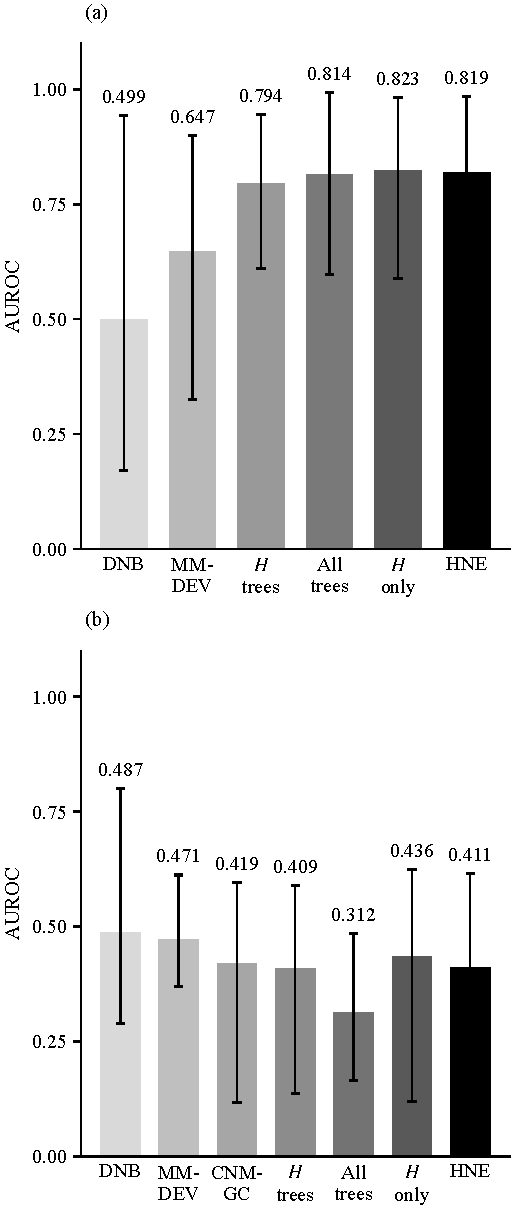
\includegraphics[width=\columnwidth]{figures/ssaqs_transfer.pdf}
\caption{Frozen-source AUROC on (a) SSAQS and (b) PMData. Error bars are participant-bootstrap intervals.}
\label{fig:ssaqs}
\end{figure}
